\chapter{Implementácia prostredia}
\section{Hracia plocha} % z coho sa sklada
\subsection{Generovanie map}% ako sa generuje, podpora ukladania, zadne zhluky, vyhody, nevyhody, 
\subsection{Vlastnosti stien} % vseobecne oba rozne vlastnosti, ake maju steny, k comu to je
\section{Jazyk hry a priebeh hry} %bison, preco
Po na čítaní všetkých robotov, ich programov sa hra klada z trojice (FrontaUdalosti f, Mapa m, ŽiviBoti b). Samotná hra prebieha tak, že pokiaľ existujú živí boti, spracuje sa nsledujúca udalost z FrontyUdalosti. O zaradenie zpať a prípadné vymazanie sa v prípade úmrtia sa objekty starajú sami.\\
Objekty = steny, boti, strely. \\
\begin{definicia}
Stav robota vzhľadom na svet charakterizuje šestica: (InstruktionStack IS , InstructionPointer IP, Hitpoints HP, CoordX x, CoordY y, Direction direct)\\
Stav robota s ohľadom na inštrukcie, ktore vykonáva, charakterizuje (InstructionStack IS, PointerStack PS, ValueStack VS, Tree t) kde IS je rovnaky ako v predchádzajúcej vete, PS zoznam pointerov na stack, VS je zásobník všetkých naloadovaných hodnôt a návratových adries z funkcií, Tree t je zoznam všetký doteraz definovaných premnných.\\
\end{definicia}

\begin{definicia} 
Pod objektami sveta rozumieme všetky prvky, ktoré svet tvoria a zároveň ho z času na čas menia, t.j. v tomto prípade strely, steny, a samotní roboti. Napríklad strela mení svet tým, že sa pohne alebo narazí, istý druh steny sa môže posunúť a pod.
\end{definicia}

\begin{definicia}
Tick je jednotka virtuálneho času sveta. Timeout je počet tickov,ktoré má robot k dispozícii na premýšľanie a tento čas nesmie prekročiť.
\end{definicia}

\begin{definicia} 
Svet je je trojica <FrontaUdalosti, Bojisko, Aktívni roboti>, kde FrontaUdalosti je fronta objektov, ktoré sú na rade, aby zmenili časť sveta. Presný spôsob definovania poradia je popísaný neskôr.
\end{definicia}
Popis jednotlivých inštrukcií a ich vplyv na svet je symbolicky popísaný takto: (bez aramterov, ktoré nemajú vplyv na svet):\\
prikazy komunikujúce so svetom:\\
$ step \left\{ \begin{array}{ll} Svet: & <f.pop()+reschedule(objekt),m.reinsert(objekt), b> \\ Bot: & < IS, IP + 1, HP, x+direct.y, y+ direct.y, direct> \end{array}\right.  $\\
$ turnLeft \left\{ \begin{array}{lc} Svet: & <f.pop()+reschedule(objekt),m, b> \\ Bot: & < IS, IP + 1, Hp, x, y, NewDirect)> \end{array}\right.  $\\
$ turnRight \left\{ \begin{array}{lc} Svet: & <f.pop()+reschedule(objekt),m, b> \\ Bot: & < IS, IP + 1, Hp, x, y, NewDirect)> \end{array}\right.  $\\
$turn  \left\{\begin{array}{lc} Svet: & <f.pop()+reschedule(objekt),m,b> \\ Bot: & <IS, IP+1, Hp, X, Y, NewDirect)> \end{array}\right. $\\
$see  \left\{\begin{array}{lc} Svet: & <f.pop()+reschedule(objekt),m,b> \\ Bot: & <IS, IP+1, Hp, X, Y, NewDirect)> \end{array}\right. $\\
$shoot \left\{\begin{array}{lc} Svet: & <f.pop()+reschedule(objekt,Strela),m,b> \\ Bot: & <IS, IP+1, Hp, X, Y, NewDirect)> \end{array}\right. $\\
\indent
Ďalšie ištrukcie vôbec nekomunikujú so svetom, preto sú uvedene oddelene. Tieto inštrukcie robot vykonáva počas svojho premýšľania. Keďze tým robot vobec nepotrebuje vedieť o objektov sveta iných než je on sám, po prevedení takýchto inštrukcií sa meni stav robota takto:\\

\begin{table}[ht]
\centering
\caption{Vnutorné príkazy robota}
\begin{tabular}{l p{5cm} }
\hline\hline
Inštrukcia & Stav bota po inštrukcii \\
store,aritmeticke+relacne operácie & $ <IS, IP[last]++, VS.add(result), t>$ \\
Call &  $ <IS.push(function_call), IP.push(Function), VS, t.add(FunctionValues)> $ \\
EndBlock & $ <IS.SetFree(block), IP[last]++, VS, t> $ \\
Destroy & $ <IS, IP[last]++, VS, t.SetInactive(name)>$ \\
Load & $ <IS, IP[last] ++, VS.push(name), t > $\\
Label & $ <IS, IP[last] ++, VS, t > $\\
Jump & $ <IS, IP-sizeof(jump), VS, t >$\\
\end{tabular}
\end{table}
%\hline
%JUMP & (InstruktionStack, Instructionpointer - LABEL, Hitpoints, X, Y, natocenie) & žiadny efekt až na preplánovanie \\ \hline               % inserting body of the table
%CALL & FunctioName & (InstruktionStack + FunctionStack, Instructionpointer = AtFunctionStack, Hitpoints, X, Y, natocenie)& žiadny efekt až na preplánovanie \\\hline
%EndFunction & (InstruktionStack - FunctionStack, Instructionpointer = AtPreviousState, Hitpoints, X, Y, natocenie)& žiadny efekt až na preplánovanie \\\hline
%\hline                              %inserts single line
%\end{tabular}
%\end{table}

\subsection{Priebeh penalizacie za instrukciu}
\begin{definicia}
Penalizáciou za inštrukciu nazývam počet tikov, ktoré robot stratí, ak inštrukciu vykoná. Pre rôzne inštrukcie môže byť rôzna.
\end{definicia}
\indent
V okamihu, keď je na rade vo fronte udalostí nejaký robot, začne robot premýšlať, akú ďalšiu akciu by mal so svetom spraviť. Podľa toho, ako dlho mu 'premýšľanie' sa potom zaradí do plánovaných objektov, viz \ref{thinking}. Dĺžka tejto akcie sa ale pre rovnaký počet inštrukcií pre dvoch rôznych botov môže a typicky bude líšiť. Je to spôsobené tým, že každá inštrukcia môže mať rozdielnu penalizáciu za vykonanie. Napríklad samostatné vykoanie inštrukcie 'step' musí byť niekoľko krát rýchlejšie ako povedzme inštrukcia, ktorá naloaduje hodnotu premennej, obzvlášť ak táto premenná už dlho loadovaná nebola. Ďalej inštrukcia, ktorá zavolá užívateľom definovanú funkciu, zaberie viac procerového času vzhladom na to, ćo musí spraviť so zásobníkom robota, a preto je táto skutočnosť zohľadnená. Podobne napríklad inštrukcie pre násobenie a delenie su zlošitejšie ako proste sčitanie a preto sú viac penalizované.\\
\indent
Robotovi môže týmto spôsobom samozrejme vypršať čas. V takom prípade, ako je naznačené na obrázku \ref{thinking} sa robot vzdá svojej možnosti interagovat so svetom a preplánuje sa. Preplánovanie prebieha tým spôsobom, že sa spočíta, kolko svojho času robot prehmrhal na myslenie, presne o toľko sa posunie v pomyselnejcasovej osi a zaradí sa vo fronte udalostí za posledného bota s rovnakým časom. Samotné inštrukcie majú penalizáciu síce nenulovú, ale najmenšiu, čo odpovedá tomu, že je to pre bota prirodzená inštrukcia a zároveň sa tým zamedzuje tomu, aby robot v prípade samých takýchto inštrukcií nepustil na radu ostatné objekty. Objekty iné ako robot majú rovnako penalizáciu, ale vždy menšiu ako je timeout. Každý takýto objekt má ale už iba funkciu interagujúcu so svetom, takze sa po prevedení tejto akcie zase preplánujú.\\
%\begin{figure}[hpt]
%\centering{
%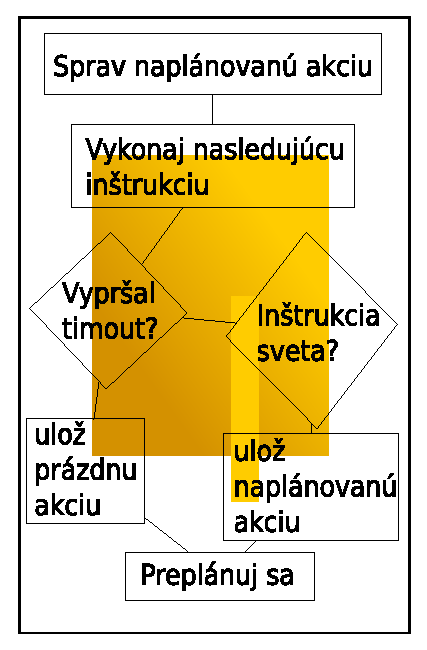
\includegraphics{thinking}
%\caption{Premýšľanie robota}
%\label{thinking}
%}
%\end{figure}

\subsection{Detekcia zacyklenia}

\section{Vlastnosti robotov}
Výsledok programu, ktorého inštrukcie robot vykonáva, je závislý na konkrétnom type robota. Typ robota je definovaný niekoľkými parametrami, ktoré si bežný užívateľ samostatne na začiatku hry definuje == UholViditelnost, PolomerViditelnosti, Obrana, Hitpoints, TypStrely, VelkostPamate==\\
\begin{table}[ht]
\caption{Vlastnosti robota}   % title of Table
\centering                          % used for centering table
\begin{tabular}{ | c | p{10cm} |}            % centered columns (4 columns)
\hline\hline                        %inserts double horizontal lines
Vlastnost & Vplyv \\   % inserts table
%heading
\hline                              % inserts single horizontal line
polomer viditeľnosti & Robot dokáže na určitú vzdialenosť rozpoznať object, táto vlastnosť určuje, koľko políčok dopredu v priamom smere( v smere, akým je bot aktualne otočený) vidí. Tento počet sa pod iným uhlom o niečo zmení,\\\hline               % inserting body of the table
uhol viditeľnosti & maximálny rozptyl viditeľnosti - robot nevidí celý kruh okolo seba, ale iba určitú výseč \\\hline
Obrana & Obranne cislo bota. Pouziva sa pri strete s nejakou prekazkou. Viz kolizie. \\\hline
Hitpoints  & životnost bota, akonahle klesne na nulu, z fronty akcií sa jeho nasledujúca akcia odstráni a robot mizne do prepadlišťa dejin\\\hline [1ex]         % [1ex] adds vertical space
Typ strely & Strela je sa definuje podobne ako samotný bot, ale ma iné parametre\\\hline
\hline                              %inserts single line
\end{tabular}
\label{table:vlastnosti}          % is used to refer this table in the text
\end{table}

\begin{table}[ht]
\caption{Vlastnosti Strely}   % title of Table
\centering                          % used for centering table
\begin{tabular}{ | c | p{10cm} |}            % centered columns (4 columns)
\hline\hline                        %inserts double horizontal lines
Vlastnost & Vplyv \\   % inserts table
%heading
\hline                              % inserts single horizontal line
Odrážavost & definuje, ako moc sa strela od steny odrazí, v podstate je to to iste ako hmotnosť\\ \hline
Rýchlosť & definuje preplanovanie vo fronte akcií\\ \hline
Hitpoints  & dolet strely, ten sa znižuje s poctom tikov a súčasne kolíziami\\ \hline
Utok & Utocne cislo bota, pouziva sa pri utok, viz kolizie \\ \hline
\hline                              %inserts single line
\end{tabular}
\end{table}

Užívateľ si typ strely definuje tak, že dostane k dispozícií určitź počet bodv a tie musí medzi jednotlive volby rozdeliť\\
Bot premýšla tak, že sa nechá bežat dovtedy, kým z jeho program nenarazí na inštrukciu, ktorá by ovplyvnila svet, alebo kým neprsiahne timeout. Ak presiahne timeout, preruší sa, preplánuje vo fronte udalostí ďalej (presnejšie o TIMEOUT tikov ďalej)\\
Velmi špeciálny je prípad, keď užívateľ nenastaví robotovi žiadnu pamať. Takýto robot nie je schopný si zapatať jedinú premennú a ani vracat návratové hodnoty, teda v kóde programu by nemali byť definované žiadne funkcie, ale iba procedúry.Je nutné povedať, že funkcie a procedúry sa v žiadnom prípade nechovajú ako premenné a teda nezaberajú robotovi pamať. Teda v tomto prípade dojde k masívnemu využitiu rekurzií. Samotne vstavané príkazy sú však vlastne funkcie, ale kedže sa nikam nemajú priradiť, ich návratová hodnota sa zahodí. Nevýhodou tohoto typu bota je však skutočnost, že nemá povolené napriklad strieľanie, pretože to je funkcia, ktorá potrebuje za každých okolností parametre.
